\chapter{Metodolog\'ia}

\label{Chapter3}

En este cap\'itulo se detallar\'an los procesos abordados para la extracci\'on y clasificaci\'on de los d\'igitos
escritos en los telegramas de las elecciones. Primero se describir\'a el proceso de obtenci\'on, limpieza y
transformaci\'on de los datos a fin de obtener un dataset con el cual entrenar. Luego, se describir\'an los procesos a
ser llevados a cabo para el dise\~{n}o experimental de los modelos.

\section{Descripci\'on de los datos}

Los telegramas fueron descargados desde la \href{https://op.elecciones.gob.ar/telegramas/generales2021/}{p\'agina
    oficial del estado argentino}. Presentan un formato est\'andar en forma de grilla donde en cada rengl\'on se encuentra
el partido pol\'itico y los votos obtenidos para diputados y senadores. En la p\'agina tambi\'en se puede descargar un
CSV donde se encuentra el {\it id} de cada telegrama y los valores digitalizados oficialmente.

\section{Extracci\'on de d\'igitos de los telegramas}

Los telegramas de las elecciones de Santa Fe presentan un formato tabular, donde cada fila representa un partido
pol\'itico y los votos obtenidos abiertos por senadores y diputados. Se debieron ejecutar m\'ultiples pasos de
extracci\'on, transformaci\'on y carga (ETL por sus siglas) de los mismos antes de poder armar un dataset con el cual
entrenar los modelos. Se utiliz\'o la librer\'ia OpenCV \parencite{opencv_library} para manipular las im\'agenes y poder llevar a cabo el proceso de ETL.

\subsection{Enderezado}
Como los telegramas son escaneados a mano, el primer paso consiste en enderezarlos. Este proceso puede realizarse
buscando el rect\'angulo de mayor \'area, calculando el \'angulo de rotaci\'on y rotando la imagen completa con la
funci\'on \verb|getRotationMatrix2D| de OpenCV.

\begin{figure}[H]
    \centering

    \tikzset{every picture/.style={line width=0.75pt}}

    \begin{tikzpicture}[x=0.75pt,y=0.75pt,yscale=-1,xscale=1]

        \draw (370,140) node  {\includegraphics[width=135pt,height=210pt]{chapter3/etl-1-rotacion.png}};
        \draw (90,140) node  {\includegraphics[width=135pt,height=210pt]{chapter3/etl-1-telegrama.png}};
        \draw    (190.8,110.6) -- (267.4,110.6) ;
        \draw [shift={(269.4,110.6)}, rotate = 180] [color={rgb, 255:red, 0; green, 0; blue, 0 }  ][line width=0.75]    (10.93,-3.29) .. controls (6.95,-1.4) and (3.31,-0.3) .. (0,0) .. controls (3.31,0.3) and (6.95,1.4) .. (10.93,3.29)   ;
        \draw (190,87.18) node [anchor=north west][inner sep=0.75pt]   [align=left] {Enderezar};

    \end{tikzpicture}

    \caption{Enderezamiento de un telegrama utilizando OpenCV.}
    \label{fig:etl-1-rotacion}
\end{figure}

\subsection{Extracci\'on de la grilla de votos}
El siguiente paso consiste en poder seleccionar la grilla de los votos y poder extraerla para seguir trabajando en
ella. Esto puede realizarse utilizando la funcion \verb|getContours| de OpenCV y qued\'andose con el contorno de mayor
\'area.

\begin{figure}[H]
    \centering
    \includegraphics[width=0.4\textwidth, height=0.3\textwidth]{chapter3/etl-2-grilla.png}
    \caption{Grilla de votos extra\'ida buscando el contorno de mayor \'area.}
    \label{fig:etl-2-grilla}
\end{figure}

\subsection{Detecci\'on de l\'ineas de la grilla de votos}
Teniendo la grilla de votos separada del telegrama, se procede a detectar las l\'ineas para poder extraer cada registro
de la misma. Si bien OpenCV posee funciones para la detecci\'on de l\'ineas, se opt\'o por utilizar un enfoque
simplificado. El mismo es similar al utilizado en \parencite{lamagna2016lectura}. Debido a que la grilla se encuentra enderezada, se puede utilizar proyecciones de los
colores sobre los ejes $x$ e $y$ para detectarlas. Al sumar todos los colores por eje, se pueden encontrar los picos
donde se encuentran las lineas horizontales y verticales. Posteriormente, se selecciona un umbral de corte por cada
eje, siendo el promedio menos dos desv\'ios est\'andar. La figura \ref{fig:etl-3-proyecciones} muestra las proyecciones
obtenidas con los umbrales por cada eje.

\begin{figure}
    \centering

    \tikzset{every picture/.style={line width=0.75pt}}

    \begin{tikzpicture}[x=0.75pt,y=0.75pt,yscale=-1,xscale=1]
        \draw (142.77,162.65) node  {\includegraphics[width=214.16pt,height=173.4pt]{chapter3/etl-3-grilla.png}};
        \draw (303.6,159.11) node [rotate=-90] {\includegraphics[width=172pt,height=46.15pt]{chapter3/etl-3-grilla-proyeccion-y.png}};
        \draw (142.5,30.77) node  {\includegraphics[width=213.75pt,height=46.15pt]{chapter3/etl-3-grilla-proyeccion-x.png}};
    \end{tikzpicture}

    \caption{Proyecciones de los ejes de la grilla. En rojo se marca el umbral de corte.}
    \label{fig:etl-3-proyecciones}
\end{figure}

Sin embargo, aunque se seleccione aquellos pixeles que se encuentren por debajo del umbral, por cada pico existe mas de
un pixel. Siguiendo con el ejemplo, en el eje $x$ se obtienen los siguientes pixeles que se encuentran en los "picos":

\begin{verbatim}
    array([    3,    4,    5,    6,    7,  100,  119,  120,  988, 
             989,  990,  991,  992, 1215, 1216, 1217, 1218, 1219, 
            1423, 1424, 1425, 1426, 1427])
\end{verbatim}

Con la estrategia del umbral no se obtienen las 4 l\'ineas que se desean detectar sobre el eje $x$. No obstante, se
puede aplicar un clustering jer\'arquico sobre los \'indices obtenidos y luego calcular el \'indice promedio de cada
cluster para tomarlo como \'unico representante. El proceso se repite de la misma manera sobre el eje $y$. Esta
\'ultima modificaci\'on sobre el trabajo realizado en \parencite{lamagna2016lectura} asegura tener un \'unico pixel por l\'inea.

\begin{figure}[H]
    \centering
    \includegraphics[width=0.4\textwidth, height=0.3\textwidth]{chapter3/etl-3-grilla-detectada.png}
    \caption{Grilla detectada (en verde) utilizando el umbral por sobre las proyecciones y su posterior agrupamiento con clustering jer\'arquico.}
    \label{fig:etl-3-grilla-detectada}
\end{figure}

\subsection{Segmentaci\'on de d\'igitos}

Una vez obtenida la grilla, se itera por cada registro obteniendo los rect\'angulos que contienen los votos, ignorando
el primer rengl\'on que contiene los t\'itulos de la grilla.

\begin{figure}[H]
    \centering
    \frame{\includegraphics[height=15pt]{chapter3/etl-4-registro-1.png}}
    \frame{\includegraphics[height=15pt]{chapter3/etl-4-registro-2.png}}
    \frame{\includegraphics[height=15pt]{chapter3/etl-4-registro-3.png}}
    \caption{Primer registro extra\'ido de la grilla de votos.}
    \label{fig:etl-4-registro}
\end{figure}

Para separar cada d\'igito en una \'unica imagen, se utiliza un an\'alisis de componentes conectados
(\verb|connectedComponents| de OpenCV) y se recortan aquellos contornos que posean de \'area entre el $5\%$ y el $70\%$
de los pixeles totales de la imagen. Los valores fueron obtenidos mediante experimentaci\'on y sirven para descartar
ruido que pueda detectar el an\'alisis de componentes conectados.

\begin{figure}[H]
    \centering
    \frame{\includegraphics[scale=0.6]{chapter3/etl-4-digito-1.png}}
    \frame{\includegraphics[scale=0.6]{chapter3/etl-4-digito-2.png}}
    \frame{\includegraphics[scale=0.6]{chapter3/etl-4-digito-3.png}}
    \caption{D\'igitos detectados en el primer bloque de votos.}
    \label{fig:etl-4-digitos}
\end{figure}

Por \'ultimo, los d\'igitos son encuadrados y se guardan junto al partido pol\'itico y al tipo de voto (senadores o
diputados) en un dataset, cuyo an\'alisis ser\'a abordado en la siguiente secci\'on.

\section{An\'alisis del dataset}

Con la extracci\'on descripta en la secci\'on anterior, se procede a hacer un an\'alisis exploratorio de los datos en
b\'usqueda de posibles errores. La tabla \ref{tab:dataset-telegramas-segmentados} muestra algunos registros del dataset
que vincula los d\'igitos extra\'idos de los telegramas con los partidos pol\'iticos.

\begin{table}[H]
    \centering
    \begin{tabular}{ccccc}
        \toprule
        Telegrama                                                               & Partido         & Tipo      & D\'igitos                                                                & \# D\'igitos \\
        \midrule
        2100100026X                                                             & Unite           & Diputados & \frame{\includegraphics[scale=0.6]{chapter3/eda/unite-diputados-1.png}}
        \frame{\includegraphics[scale=0.6]{chapter3/eda/unite-diputados-2.png}}
        \frame{\includegraphics[scale=0.6]{chapter3/eda/unite-diputados-3.png}} & 3                                                                                                                     \\
        2100100026X                                                             & Unite           & Senadores & \frame{\includegraphics[scale=0.08]{chapter3/eda/unite-senadores-1.png}}
        \frame{\includegraphics[scale=0.6]{chapter3/eda/unite-senadores-2.png}}
        \frame{\includegraphics[scale=0.6]{chapter3/eda/unite-senadores-3.png}}
        \frame{\includegraphics[scale=0.6]{chapter3/eda/unite-senadores-4.png}} & 4                                                                                                                     \\
        2100100067X                                                             & Frente de Todos & Diputados & \frame{\includegraphics[scale=0.6]{chapter3/eda/todos-diputados-1.png}}
        \frame{\includegraphics[scale=0.6]{chapter3/eda/todos-diputados-2.png}}
        \frame{\includegraphics[scale=0.6]{chapter3/eda/todos-diputados-3.png}}
        \frame{\includegraphics[scale=0.6]{chapter3/eda/todos-diputados-4.png}} & 4                                                                                                                     \\
        2100100067X                                                             & Frente de Todos & Senadores & \frame{\includegraphics[scale=0.6]{chapter3/eda/todos-senadores-1.png}}
        \frame{\includegraphics[scale=0.6]{chapter3/eda/todos-senadores-2.png}}
        \frame{\includegraphics[scale=0.6]{chapter3/eda/todos-senadores-3.png}} & 3                                                                                                                     \\
        \bottomrule

    \end{tabular}
    \caption{Ejemplo de registros del dataset. Cada fila representa un voto.}
    \label{tab:dataset-telegramas-segmentados}
\end{table}

El lector podr\'a darse cuenta que existen errores en el cuadro anterior. En primer lugar, en la columna donde
s\'olamente deben haber las im\'agenes de los d\'igitos existe una con una l\'inea en el segundo registro. Por otro
lado, tambi\'en existen d\'igitos mal escritos como los que se encuentran en los dos \'ultimos registros. Para limpiar
estas extracciones incorrectas, se calculan dos columnas las cuales contienen las proporciones m\'inimas y m\'aximas de
pixeles blancos en las im\'agenes por cada voto. La figura \ref{fig:histogramas-min-max-prop-blanco} muestra los
histogramas generales de las mismas.

\begin{figure}[H]
    \centering
    \begin{subfigure}[h]{0.48\textwidth}
        \includegraphics[width=1\textwidth]{chapter3/eda/hist-min-prop-blanco.png}
        \caption{Histograma de la proporci\'on m\'inima de pixeles blancos en un voto.}
        \label{fig:histograma-min-prop-blanco}
    \end{subfigure}
    \hfill
    \begin{subfigure}[h]{0.48\textwidth}
        \includegraphics[width=1\textwidth]{chapter3/eda/hist-max-prop-blanco.png}
        \caption{Histograma de la proporci\'on m\'axima de pixeles blancos en un voto.}
        \label{fig:histograma-max-prop-blanco}
    \end{subfigure}
    \caption{Histogramas de proporciones de pixeles blancos por voto.}
    \label{fig:histogramas-min-max-prop-blanco}
\end{figure}

La cola derecha de la distribuci\'on de \ref{fig:histograma-max-prop-blanco} presenta un pico anormal en el extremo
cercano a 1. Al eliminar aquellas im\'agenes de d\'igitos que posean mas de un $95\%$ de pixeles blancos, se logran
descartar los casos de l\'ineas como la vista en el cuadro \ref{tab:dataset-telegramas-segmentados}. Por el contrario,
al eliminar aquellas im\'agenes que posean menos del $50\%$ de pixeles blancos, se logran descartar los casos de
escritura incorrecta.

El siguiente punto a analizar es el tama\~{n}o de las im\'agenes. Como fue mostrado en el cuadro
\ref{tab:dataset-telegramas-segmentados}, las im\'agenes no fueron estandarizadas en un tama\~{n}o est\'andar. De
manera an\'aloga a la variable de proporci\'on de pixeles blancos, se calculan las variables m\'inimo y m\'aximo
tama\~{n}o por voto. La tabla \ref{tab:describe-min-max-size} muestra los estad\'isticos descriptivos de las mismas.

\begin{table}[H]
    \centering
    \begin{tabular}{crrrrr}
        \toprule
        Variable            & Promedio & Desv\'io & M\'inimo & Mediana & M\'aximo \\
        \midrule
        Tama\~{n}o m\'inimo & 38.35    & 9.61     & 13       & 37      & 621      \\
        Tama\~{n}o m\'aximo & 44.80    & 10.73    & 18       & 43      & 621      \\
        \bottomrule
    \end{tabular}
    \caption{Estad\'isticos descriptivos del m\'inimo y m\'aximo tama\~{n}o de las im\'agenes de los votos.}
    \label{tab:describe-min-max-size}
\end{table}

Al analizar los valores extremos, se encuentran telegramas que fueron cargados de forma incorrecta (ver anexo
\ref{anexo:telegrama-erroneo}) o con caligraf\'ia en la cual los n\'umeros se encuentran unidos y no pueden ser
separados por el an\'alisis de componentes conectados de OpenCV (ver anexo \ref{anexo:telegrama-numeros-juntos}). Se
eliminan estos casos filtrando por aquellos registros que se encuentren por fuera de la media +- 4 desv\'ios
est\'andar.

Concluida la etapa de an\'alisis y limpieza, se exportan los d\'igitos en un formato similar al dataset {\it MNIST} con
la etiqueta que oficialmente fue registrada en las elecciones del 2021. El mismo ser\'a nombrado como {\it TDS}
(dataset de telegramas) de aqu\'i en adelante. El mismo posee un total de 170.718 im\'agenes de d\'igitos cuadradas con
sus dimensiones orginales, es decir, no se encuentran estandarizados en una dimension espec\'ifica. Esto \'ultimo es
adrede ya que puede servir para mejorar el dataset en futuros trabajos.

\begin{figure}[H]
    \centering
    \includegraphics[width=0.5\textwidth]{chapter3/tds.png}
    \caption{Dataset TDS de d\'igitos.}
    \label{fig:tds}
\end{figure}

\section{Dise\~{n}o experimental}

% TODO: no me deja referenciar a tllib de la bib, no se que por que rompe.
Los experimentos fueron programados en Python mediante la librer\'ia \href{https://pytorch.org/}{PyTorch} \parencite{NEURIPS2019_9015} y \href{https://github.com/thuml/Transfer-Learning-Library}{TLLIB} para aplicar las t\'ecnicas
de adaptaci\'on de dominio.

Se entrenaron redes ResNet-50 \parencite{he2016deep} y LeNet-8 \parencite{lecun1998gradient} por cada una de las t\'ecnicas de adaptaci\'on de dominio descriptas en el cap\'itulo
\ref{Chapter2}. Como modelo baseline, se entrenaron ambas redes sin ninguna t\'ecnica de adaptaci\'on.

\subsection{Metodolog\'ia de entrenamiento}

Para entrenar modelos mediante adaptaci\'on de dominio, se precisan dos datasets: el de origen que se encuentra
etiquetado y el de destino sin etiquetar. Los experimentos llevados a cabo utilizan el {\it MNIST} como origen y el
    {\it TDS} como destino. En cada iteraci\'on de entrenamiento, se provee de un batch de 1024 im\'agenes del dataset
origen y otro del de destino. Se realizaron 3 particiones de cada uno:

\begin{itemize}
    \item Entrenamiento (70\% de cada dataset): utilizado para entrenar la LeNet-8 y ResNet-18 en cada \'epoca.
    \item Validaci\'on (15\% de cada dataset): utilizado para calcular los mejores hiperpar\'ametros del modelo.
    \item Test (15\% de cada dataset): utilizado para calcular las m\'etricas y gr\'aficos finales del modelo entrenado.
\end{itemize}

Los modelos se entrenaron utilizando Stochastic Gradient Descent (SGD) \parencite{sutskever2013importance} utilizando nesterov, 0.9 como momento y 0.001 de weight decay.

\subsection{Selecci\'on y optimizaci\'on del modelo}

La optimizaci\'on de hiperpar\'ametros se realiz\'o utilizando la librer\'ia Optuna \parencite{optuna_2019}. Se ejecutaron 30 rondas de optimizaci\'on con 10 \'epocas de entrenamiento por cada experimento.
En cada uno de los experimentos, se optimizaron los hiperpar\'ametros para minimizar el loss de cada modelo. El cuadro
\ref{tab:rangos-hiperparametros} muestra los rangos b\'usqueda.

\begin{table}[H]
    \centering
    \begin{tabular}{l|cccccc}
        \toprule
                   & {\it DANN}  & {\it ADDA}  & {\it DANN+BSP} & {\it MDD}   & {\it AFN}    & {\it Sin AD} \\
        \midrule
        $\eta_0$   & [1e-4, 0.1] & [1e-4, 0.1] & [1e-4, 0.1]    & [1e-4, 0.1] & [1e-4, 0.1]  & [1e-4, 0.1]  \\
        $\lambda$  & [0.5, 2]    & [0.5, 2]    & [0.5, 2]       & [0.5, 2]    & [0.001, 0.1] & -            \\
        $\beta$    & -           & -           & [1e-5, 0.1]    & -           & [0.0, 0.1]   & -            \\
        $\gamma$   & -           & -           & -              & [1, 10]     & -            & -            \\
        $\Delta_r$ & -           & -           & -              & -           & [0.01, 5]    & -            \\
        \# Blocks  & -           & -           & -              & -           & [1, 4]       & -            \\
        Dropout    & -           & -           & -              & -           & [0.3, 0.7]   & -            \\
        \bottomrule
    \end{tabular}
    \caption{Rango de hiperpar\'ametros optimizados. $^{*}$LR refiere a "learning rate". $^{**}$T-O refiere a "trade-off".}
    \label{tab:rangos-hiperparametros}
\end{table}

Se implement\'o una disminuci\'on del learning rate en cada iteraci\'on de cada \'epoca, mediante la f\'ormula
\ref{eq:learning-rate}. Se mantuvieron constantes los valores de $\gamma=0.001$ y $\theta = 0.25$.

\begin{equation}
    \eta(t) = \eta_0 * (1 + \gamma * t)^{-\theta}
    \label{eq:learning-rate}
\end{equation}

\section{M\'etricas de evaluaci\'on}

Los modelos optimizados ser\'an evaluados con distintas m\'etricas en tiempo de test, descriptas en las siguientes
sub-secciones del cap\'itulo. Las mismas pretenden evaluar qu\'e tan buenos son los modelos respecto a la tarea de
clasificaci\'on y qu\'e capacidad de adaptaci\'on de dominio poseen.

\subsection{Métricas de clasificación}
\subsubsection{Accuracy}

La m\'etrica de {\it accuracy} permite identificar qu\'e tan cerca o lejos un conjunto de observaciones se encuentra
respecto a los valores reales. Es el ratio de predicciones correctas sobre las totales.

\begin{equation}
    Accuracy(y, \hat{y}) = \frac{1}{n} \sum_{i=0}^{n-1} 1(\hat{y_{i}}=y_{i})
\end{equation}

Donde:
\begin{itemize}
    \item $n$: es la cantidad de observaciones totales.
    \item $y_{i}$: es el valor de la ${i}$-\'esima observaci\'on correspondiente al real.
    \item $\hat{y_{i}}$: es el valor predicho para la ${i}$-\'esima observaci\'on.
    \item $1(x)$: es la funci\'on indicador.
\end{itemize}

\subsubsection{$F_{1}$}

La m\'etrica $F_{1}$ es una media arm\'onica de otras dos: {\it precisi\'on} y {\it recall}. De manera simplificada, la
primera muestra la capacidad del modelo de no etiquetar como positivo una obsevaci\'on que es negativa y la segunda
muestra la capacidad del modelo de encontrar todas las observaciones positivas.

La {\it precisi\'on} consiste en calcular el ratio de predicciones positivas correctas de la clase respecto al total de
predicciones positivas de la clase.

\begin{equation}
    Precision(y, \hat{y}) = \frac{TP}{TP + FP}
\end{equation}

Donde:
\begin{itemize}
    \item $TP$: es la cantidad de verdaderos positivos.
    \item $FP$: es la cantidad de falsos positivos.
\end{itemize}

Por otro lado, el {\it recall} consiste en calcular el ratio de predicciones positivas correctas de la clase respecto
al total de predicciones correctas de la clase.

\begin{equation}
    Recall(y, \hat{y}) = \frac{TP}{TP + FN}
\end{equation}

Donde:
\begin{itemize}
    \item $TP$: es la cantidad de verdaderos positivos.
    \item $FN$: es la cantidad de falsos negativos.
\end{itemize}

Las dos m\'etricas mencionada anteriormente pueden ser combinadas en una sola denominada $F_{\beta}$. El valor de
$\beta$ permite asignar un peso distinto a la precisi\'on o al recall dentro del promedio arm\'onico. Cuando $\beta=1$,
ambas poseen el mismo peso.

\begin{equation}
    F_{\beta}(y, \hat{y}) = (1 + \beta^2) \times \frac{precision(y, \hat{y}) \times recall(y, \hat{y})}{\beta^2 \times precision(y, \hat{y}) + recall(y, \hat{y})}
\end{equation}

El rango de valores es de $[0, 1]$, donde 1 corresponde a un clasificador que funciona sin errores.

\subsubsection{Intersecci\'on sobre uni\'on}

Otra forma de medir el clasificador es mediante la {\it intersecci\'on sobre uni\'on} (IoU por sus siglas en ingl\'es).
Consta de calcular la cantidad de d\'igitos \'unicos predichos por sobre la cantidad de d\'igitos \'unicos reales. Por
ejemplo, para un telegrama y un partido el clasificador predice 189 votos cuando lo real es 180. Entonces, el {\it IoU}
viene dado por:

\begin{align}
    IoU(\{1, 8, 0\}, \{1, 8, 9\}) & = \frac{\lvert\{1, 8, 0\} \bigcap \{1, 8, 9\}\rvert}{\lvert\{1, 8, 0\} \bigcup \{1, 8, 9\}\rvert} \nonumber \\
                                  & = \frac{\lvert\{1, 8\}\rvert}{\lvert\{1, 8, 0, 9\}\rvert}                                         \nonumber \\
                                  & = \frac{2}{4}                                                                     \nonumber                 \\
                                  & = 0.5
\end{align}

De forma general: sea $y_{i}$ el d\'igito $i$-\'esimo del voto real $y$ de longitud $n$, $\hat{y_{j}}$ el d\'igito
$j$-\'esimo del voto predicho por el modelo $\hat{y}$ de longitud $m$, entonces la m\'etrica viene dada por:

\begin{equation}
    IoU(y, \hat{y}) = \frac{\lvert \{y_{i}\} \bigcap \{\hat{y_{j}}\}\rvert}{\lvert \{y_{i}\} \bigcup \{\hat{y_{j}}\}\rvert} \forall i \in \{1, \cdots, n\}, \forall j \in \{1, \cdots, m\}
\end{equation}

\subsection{Métricas de adaptación}
\subsubsection{Distancia $\mathcal{A}$}

La distancia $\mathcal{A}$ mide la similaridad entre dos distribuciones. Puede ser utilizada para analizar los espacios
latentes de clasificadores en problemas de adaptaci\'on de dominio \parencite{ben2006analysis}. La m\'etrica viene dada por:

\begin{equation}
    dist_\mathcal{A} = 2 (1-2\epsilon)
\end{equation}

Donde $\epsilon$ es el error en test de un clasificador entrenado para discriminar el dominio de origen del de destino.
Cuando el error de clasificaci\'on es bajo, significa que hay diferencias significativas entre las dos distrubiones,
haciendo que $dist_\mathcal{A}$ sea grande y vice versa.

En la figura \ref{fig:ejemplos-dist-a} se muestran posibles casos de distribuciones de dominios. En la sub-figura
\ref{fig:dominios-distintos} las distribuciones de dominios son significativamente diferentes entre si, por lo tanto
$dist_\mathcal{A} \approx 2$. Por el contrario, en la sub-figura \ref{fig:dominios-similares} las distribuciones de
dominios son similares entre si, por lo que se espera que $dist_\mathcal{A} \approx 0$.

\begin{figure}[H]
    \centering
    \begin{subfigure}[h]{0.46\textwidth}
        \centering
        \tikzset{every picture/.style={line width=0.75pt}}
        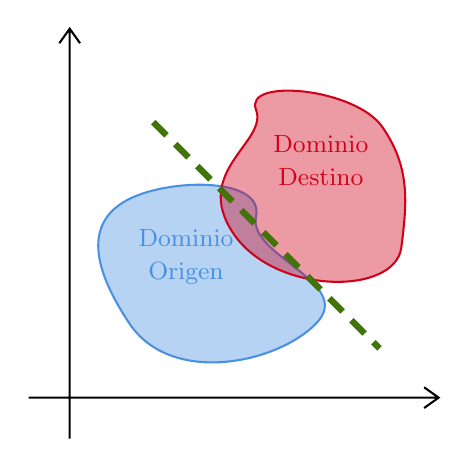
\begin{tikzpicture}[x=0.75pt,y=0.75pt,yscale=-1,xscale=1]
            \draw  (0,177.75) -- (197.5,177.75)(19.75,0) -- (19.75,197.5) (190.5,172.75) -- (197.5,177.75) -- (190.5,182.75) (14.75,7) -- (19.75,0) -- (24.75,7)  ;
            \draw  [color={rgb, 255:red, 74; green, 144; blue, 226 }  ,draw opacity=1 ][fill={rgb, 255:red, 74; green, 144; blue, 226 }  ,fill opacity=0.4 ] (48.5,82) .. controls (68.5,72) and (113.5,71.5) .. (109.5,90.5) .. controls (105.5,109.5) and (157.5,122.5) .. (138.5,142) .. controls (119.5,161.5) and (68.5,172) .. (48.5,142) .. controls (28.5,112) and (28.5,92) .. (48.5,82) -- cycle ;
            \draw  [color={rgb, 255:red, 208; green, 2; blue, 27 }  ,draw opacity=1 ][fill={rgb, 255:red, 208; green, 2; blue, 27 }  ,fill opacity=0.4 ] (109.5,39) .. controls (103.5,23.5) and (157.5,28.5) .. (170.5,47.5) .. controls (183.5,66.5) and (182.5,82.5) .. (179.5,105.5) .. controls (176.5,128.5) and (118.5,128.5) .. (98.5,98.5) .. controls (78.5,68.5) and (115.5,54.5) .. (109.5,39) -- cycle ;
            \draw (115,50) node [anchor=north west][inner sep=0.75pt]  [color={rgb, 255:red, 208; green, 2; blue, 27 }  ,opacity=1 ] [align=left] {\begin{minipage}[lt]{36.4pt}\setlength\topsep{0pt}
                    \begin{center}
                        {\small Dominio}\\{\small Destino}
                    \end{center}

                \end{minipage}};
            \draw (50,95) node [anchor=north west][inner sep=0.75pt]  [color={rgb, 255:red, 74; green, 144; blue, 226 }  ,opacity=1 ] [align=left] {\begin{minipage}[lt]{36.4pt}\setlength\topsep{0pt}
                    \begin{center}
                        {\small Dominio}\\{\small Origen}
                    \end{center}

                \end{minipage}};
            \draw [color={rgb, 255:red, 65; green, 117; blue, 5 }  ,draw opacity=1 ][line width=2.25]  [dash pattern={on 6.75pt off 4.5pt}]  (60,45) -- (169,154) ;
        \end{tikzpicture}
        \caption{Dominios distintos, discriminables.}
        \label{fig:dominios-distintos}
    \end{subfigure}
    \hfill
    \begin{subfigure}[h]{0.46\textwidth}
        \centering
        \tikzset{every picture/.style={line width=0.75pt}}

        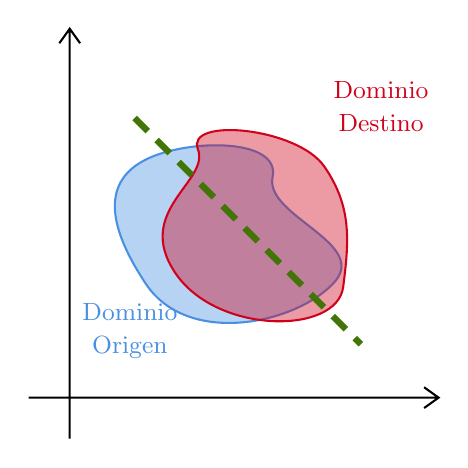
\begin{tikzpicture}[x=0.75pt,y=0.75pt,yscale=-1,xscale=1]
            \draw  (1,179.75) -- (198.5,179.75)(20.75,2) -- (20.75,199.5) (191.5,174.75) -- (198.5,179.75) -- (191.5,184.75) (15.75,9) -- (20.75,2) -- (25.75,9)  ;
            \draw  [color={rgb, 255:red, 74; green, 144; blue, 226 }  ,draw opacity=1 ][fill={rgb, 255:red, 74; green, 144; blue, 226 }  ,fill opacity=0.4 ] (57.5,65) .. controls (77.5,55) and (122.5,54.5) .. (118.5,73.5) .. controls (114.5,92.5) and (166.5,105.5) .. (147.5,125) .. controls (128.5,144.5) and (77.5,155) .. (57.5,125) .. controls (37.5,95) and (37.5,75) .. (57.5,65) -- cycle ;
            \draw  [color={rgb, 255:red, 208; green, 2; blue, 27 }  ,draw opacity=1 ][fill={rgb, 255:red, 208; green, 2; blue, 27 }  ,fill opacity=0.4 ] (82.5,60) .. controls (76.5,44.5) and (130.5,49.5) .. (143.5,68.5) .. controls (156.5,87.5) and (155.5,103.5) .. (152.5,126.5) .. controls (149.5,149.5) and (91.5,149.5) .. (71.5,119.5) .. controls (51.5,89.5) and (88.5,75.5) .. (82.5,60) -- cycle ;
            \draw [color={rgb, 255:red, 65; green, 117; blue, 5 }  ,draw opacity=1 ][line width=2.25]  [dash pattern={on 6.75pt off 4.5pt}]  (52,45) -- (161,154) ;

            \draw (24,133) node [anchor=north west][inner sep=0.75pt]  [color={rgb, 255:red, 74; green, 144; blue, 226 }  ,opacity=1 ] [align=left] {\begin{minipage}[lt]{36.4pt}\setlength\topsep{0pt}
                    \begin{center}
                        {\small Dominio}\\{\small Origen}
                    \end{center}

                \end{minipage}};
            \draw (145,26) node [anchor=north west][inner sep=0.75pt]  [color={rgb, 255:red, 208; green, 2; blue, 27 }  ,opacity=1 ] [align=left] {\begin{minipage}[lt]{36.4pt}\setlength\topsep{0pt}
                    \begin{center}
                        {\small Dominio}\\{\small Destino}
                    \end{center}

                \end{minipage}};
        \end{tikzpicture}

        \caption{Dominios similares, no discriminables.}
        \label{fig:dominios-similares}
    \end{subfigure}

    \caption{Ejemplos de distribuciones de dominios.}
    \label{fig:ejemplos-dist-a}
\end{figure}

Durante el proyecto se utiliza como clasificador una regresi\'on log\'istica a fin de calcular la distancia
$\mathcal{A}$.

\subsubsection{Discrepancia M\'axima Promedio}

\cite{gretton2012kernel} introduce un test estad\'istico que permite identificar si una distribuci\'on es distinta a
otra llamado Discrepancia M\'axima Promedio (MMD por sus siglas en ingl\'es). El test permite analizar qu\'e tan
bien el modelo permite adaptar el aprendizaje del dataset de origen con el de destino. Cuando el test resulte no
significativo se puede concluir que los espacios latentes generados por el modelo para ambos datasets difieren y no se
logr\'o una buena adaptaci\'on.

De manera formal, dado un espacio $\mathbb{R}^d$ y muestras IID $X_i \in \mathbb{R}^d, i=1,...N_X$ de la distribuci\'on
$X \sim P_X$ y $Y_i \in \mathbb{R}^d, i=1,...N_Y$ de la distribuci\'on $Y \sim P_Y$, se quiere demostrar que $P_X$ es
distinto de $P_Y$. El test planteado es:

\begin{align}
    H_0) & P_X \neq P_Y \nonumber \\
    H_1) & P_X = P_Y
\end{align}

Se utiliz\'o la librer\'ia \href{https://github.com/torchdrift/torchdrift/}{TorchDrift} para implementarlo en la
evaluaci\'on de los modelos. La misma utiliza una variaci\'on de test MMD utilizando un kernel RBF para aproximar $P_X$
y $P_Y$.

TODO: Completar como se calcula el score del test